\documentclass{article}

\textwidth=6.5in
\textheight=8.5in
\voffset=-54pt
\oddsidemargin=0in
\evensidemargin=0in
\setlength{\parskip}{8pt}
\setlength{\parindent}{0pt}

\usepackage{amsmath, amssymb}
\usepackage{ifthen}

\usepackage[inline]{enumitem}
\setlist{topsep=0pt, parsep=8pt}

\usepackage[rgb,table]{xcolor}\convertcolorsUfalse
\usepackage{graphicx}

% change hyperref options
\PassOptionsToPackage{hyphens}{url}
\usepackage[bookmarks,colorlinks,linkcolor=black,citecolor=blue,pdfstartview=FitH,urlcolor=blue]{hyperref}
\hypersetup{pdfpagemode=UseNone}
\usepackage{bookmark}

\usepackage{graphicx}
\usepackage{multicol}
\usepackage{framed}
\usepackage{array}

\usepackage{icomma}

\usepackage{pifont}

\usepackage{soul}

\usepackage{pgfplots}
\pgfplotsset{compat=1.18}  
\pgfplotscreateplotcyclelist{mycolor}{black, blue, red, green!70!black, magenta, purple, cyan, orange }  
\pgfplotsset{
  disabledatascaling,
  cycle list=tikzcolor, 
  axis lines=middle,
  every axis plot/.style={no marks, thick},
  every axis/.style={
    enlarge x limits=false,
    enlarge y limits=auto,
    xlabel style={at={(current axis.right of origin)},anchor=west},
    ylabel style={at={(current axis.above origin)},anchor=south},
    % extra x and y ticks for asymptotes
    extra x tick style={grid=major, grid style={dashed,black}},
    extra y tick style={grid=major, grid style={dashed,black}},
    /pgf/number format/1000 sep={},
  },    
  tick label style = {font=\footnotesize, fill=\currentbgcolor, inner sep=0pt},    
  xticklabel shift=1pt,    
  scaled ticks=false,
  scaled y ticks=false,
  unbounded coords=jump,
  samples=101,
  minor tick length=0,
  scatter/classes={
    open={mark=*,draw=black,fill=white, mark size=2, thin},
    closed={mark=*,draw=black,fill=black, mark size=2, thin}
  },
  width=3in,
}
\pgfplotsset{open/.style={only marks, mark=*, fill=white, thin, mark size=2}}
\pgfplotsset{closed/.style={only marks, mark=*, draw=black, fill=black,
    thin, mark size=2}}
\pgfplotsset{labeled/.style={nodes near coords, only marks, mark=*, draw=black, fill=black, thin, mark size=2, point meta=explicit symbolic}}

\usepackage{tikz}
\usetikzlibrary{
  matrix,%
  % enables the snake paths
  decorations.pathmorphing,%
  % enables bigger arrows
  decorations.markings,%
  decorations.pathreplacing,%
  decorations.text,%
  calc,%
  patterns,%
  shapes.geometric,%
  arrows,
  decorations.shapes,
  positioning,
  plotmarks,
  intersections
}
\tikzset{>=latex} % sets default arrow type in tikz
\tikzset{font=\normalsize}
\tikzset{mark size=1.5pt, mark options=thin}
\tikzset{pin distance=4pt,
  every pin edge/.style={<-, thin, shorten <= -2pt}}

\interfootnotelinepenalty=10000
\renewcommand{\thefootnote}{(\arabic{footnote})}

\usepackage{multirow, bigdelim}

% change to \usepackage[sols]{handout} to see solutions
\usepackage{handout}
\renewcommand{\workshopnote}{CA Notes.}    

\providecommand{\check}{}
\renewcommand{\check}{\ifmmode{\text{ \ding{51} }}\else{\ding{51} }\fi}

\newcommand\iscurrentenumi[1]{%
  \ifthenelse{\equal{#1}{\theenumi}}{}{#1}}
\setenumerate[1]{ref=\#\arabic*}
\setenumerate[2]{ref=\protect\iscurrentenumi{\theenumi}(\alph*)}
\newcommand\enumiiprefix[2]{%
  \ifthenelse{{\equal{#1}{\theenumi}}\AND{\equal{#2}{(\alph{enumii})}}}{}{}%
  \ifthenelse{{\equal{#1}{\theenumi}}\AND{\NOT{\equal{#2}{(\alph{enumii})}}}}{#2}{}%
  \ifthenelse{\equal{#1}{\theenumi}}{}{#1#2}%
}
\setenumerate[3]{ref=\protect\enumiiprefix{\theenumi}{(\alph{enumii})}\roman*}

\newlength{\tipmargin}
\makeatletter

\renewenvironment{framed}{
  \setlength{\tipmargin}{\textwidth-\linewidth}
  \advance\@totalleftmargin-\tipmargin
  \def\FrameCommand{\hspace{\tipmargin}\fbox}%
  \advance\linewidth\tipmargin
  \MakeFramed {\advance\hsize-\width \FrameRestore}%
}
{\endMakeFramed}

\makeatother

\renewcommand{\answer}[1]{#1}

\definecolor{purple}{rgb}{0.5,0,1.0}

\newcommand{\concaveup}{\raisebox{-1pt}{\tikz[x=0.075cm,y=0.075cm] \draw (-2, 4) parabola bend (0, 0) (2, 4);}}
\newcommand{\concavedown}{\raisebox{-1pt}{\tikz[x=0.075cm,y=0.075cm] \draw (-2, -4) parabola bend (0, 0) (2, -4);}}

\usepackage{fancyhdr}
\lhead{\textcolor{white}{This content is protected and may not be shared, uploaded, or distributed.}}
\rhead{}
\rfoot{\vspace*{\fill}\footnotesize\textcopyright{} \emph{Harvard Math Ma}}
\renewcommand{\headrulewidth}{0pt}
\pagestyle{fancy}
\begin{document}

\htitle{Workshop 4}

\begin{workshop}
  Start the workshop with the Google Slides about using practice exams effectively. Please check out the slides before workshop to see whether you have questions about them. 

  Slide 12 has an animation. (To see the animation, click Slideshow in the top right.) Encourage students to use colors in the way suggested by the slide: first try to solve the problem in one color. When they get stuck and use resources, switch to a different color. That way, they can easily flip through their completed practice exam to see how much they were able to do by themselves. 
\end{workshop}

\begin{enumerate}
\item  \label{2023-e1practice-graphing-1-v1} 

  Suppose we know the following about a function $f$:
  \begin{itemize}[nosep]
  \item $f$ is continuous on $(-\infty, \infty)$
  \item $f'(x) = x^3 + 3x^2$
  \item $f''(x) = 3x^2 + 6x$
  \end{itemize}
  \begin{enumerate}

  \item
    \begin{problem}[\stretch{0.25}]
      Where is $f'(x) = 0$? 
    \end{problem}

    \begin{solution}
      Since $f'(x) = x^3 + 3x^2 = x^2 (x + 3)$, we have $f'(x) = 0$ when $x = \boxed{0, -3}$. 
    \end{solution}

  \item
    \begin{problem}[\vfill]
      Where is $f$ increasing? Where is $f$ decreasing? What are the turning points of $f$?
    \end{problem}

    \begin{solution}
      We can answer this by making a sign chart for $f'$. We already saw that $f' = 0$ when $x = 0, -3$. Testing points in each section of the sign chart, we get
      \begin{center}
        \begin{tikzpicture}
          \begin{axis}[axis y line=none, x axis line style={-}, xtick={-3, 0}, ymin=-2, ymax=2, height=1.25in, width=3in, clip=false]
            \addplot+[domain=-9:3, very thin]{0};
            \draw(-9, 0) node[anchor=south west] {$f$};%
            \draw (-9, -1.5) node[right] {sign of $f'$};%
            \draw (-4.5, -1.5) node{$-$};%
            \draw[->, xshift=2pt] (-5.7, 1.5) -- (-3.3, 0.5);%
            \draw (-1.5, -1.5) node{$+$};%
            \draw[->, xshift=2pt] (-2.7, 0.5) -- (-0.3, 1.5);%
            \draw (1.5, -1.5) node{$+$};%
            \draw[->, xshift=2pt] (0.3, 1.5) -- (2.7, 2.5);%
            \draw[->, xshift=2pt] (-3.3, 0.5) -- (-2.7, 0.5);%
            \draw[->, xshift=2pt] (-0.3, 1.5) -- (0.3, 1.5);%
          \end{axis}
        \end{tikzpicture}
      \end{center}
      So, $f$ is \fbox{decreasing on $(-\infty, -3)$ and increasing on $(-3, \infty)$}.

      Therefore, the \fbox{only turning point point is $-3$}. 
    \end{solution}

  \item
    \begin{problem}[\vfill]
      Where is $f$ concave up? Where is $f$ concave down? What are the inflection points of $f$? 
    \end{problem}

    \begin{solution}
      We can answer this by making a sign chart for $f''$. We have $f''(x) = 3x^2 + 6x = 3x (x + 2)$, and this is 0 when $x = 0, -2$. Testing a point in each section, we get the following sign chart:
      \begin{center}        
        \begin{tikzpicture}
          \begin{axis}[axis y line=none, x axis line style={-}, xtick={-2, 0}, ymin=-2, ymax=2, height=1.25in, width=3in, clip=false]
            \addplot+[domain=-6:2, very thin]{0};
            \draw(-6, 0) node[anchor=south west] {$f$};%
            \draw (-6, -1.5) node[right] {sign of $f''$};%
            \draw (-3, -1.5) node{$+$};%
            \draw (-1, -1.5) node{$-$};%
            \draw (1, -1.5) node{$+$};%
            \draw (-3, 1) node{\concaveup};%
            \draw (-1, 1) node{\concavedown};%
            \draw (1, 1) node{\concaveup};%
          \end{axis}
        \end{tikzpicture}
      \end{center}
      So, \fbox{$f$ is concave up on $(-\infty, -2)$ and $(0, \infty)$ and concave down on $(-2, 0)$}.

      Therefore, the \fbox{inflection points are $0, -2$}. 
    \end{solution}

  \item
    \begin{problem}[\stretch{2}]
      Sketch a possible graph of $f$. 
    \end{problem}

    \begin{solution}
      Let's start to the left of $x = -3$. 
      Since we aren't told any values of $f$, we can start the graph at any height. We should draw something that's decreasing and concave up until $x = -3$, then switch to increasing and concave up. At $x = -2$, the graph should switch to increasing and concave down. Remember we saw that $f'(0) = 0$, so the graph should flatten out to a horizontal slope there. Then, it's increasing and concave up after that. So, here's a possibility:
      \begin{center}
        \answer{
          \begin{tikzpicture}
            \begin{axis}[xtick={-3, -2, 0}, ytick=\empty, enlarge y limits=false, ymin=0]
              \addplot+[domain=-4:2]{x^4/4+x^3+8};
            \end{axis}
          \end{tikzpicture}
        }
      \end{center}
      Any vertical shift of this would also be correct. 
    \end{solution}

  \item
    \begin{workshop}
      This is especially to prompt students to see whether they've drawn a graph with $f'(0) = 0$. 
    \end{workshop}

    \begin{problem}[\newpage]
      \check Is your graph consistent with your answers to the previous parts? 
    \end{problem}
  \end{enumerate}

\item  

  A computer animator is trying to make an animation of a rabbit rushing back and forth along a sidewalk. She decides to model the rabbit's velocity as a function of time time as shown in the following graph, where time is measured in seconds and velocity is measured in meters per second.
  \begin{center}
    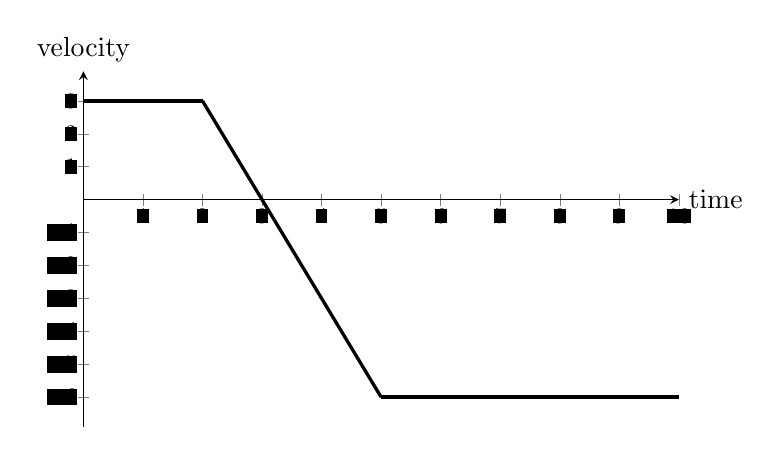
\begin{tikzpicture}
      \begin{axis}[cycle list=black, xtick={1, 2, ..., 10}, ytick={-6, -5, ..., 6}, every axis plot/.style={very thick}, xlabel=time, ylabel=velocity, width=3.6in, height=2.4in]
        \addplot+[domain=0:2]{3}; %
        \addplot+[domain=2:5]{3-3*(x-2)}; %
        \addplot+[domain=5:10]{-6}; %
      \end{axis}
    \end{tikzpicture}
  \end{center}
  Here, positive velocities indicate that the rabbit is heading east; negative velocities indicate that the rabbit is heading west.

  Let $r(t)$ be the rabbit's position (measured in meters) at time $t$ (measured in seconds).

  \begin{enumerate}
  \item
    \begin{problem}[\vfill]
      Where in $(0, 10)$ is $r(t)$ increasing? Where in $(0, 10)$ is $r(t)$ decreasing?
    \end{problem}

  \item
    \begin{problem}[\vfill]
      Where in $(0, 10)$ is $r(t)$ concave up? Where in $(0, 10)$ is $r(t)$ concave down? 
    \end{problem}

  \item
    \begin{problem}[\nstretch{0.5}]
      Is the graph of $r(t)$ steeper when $t = 1$ or when $t = 9$?
    \end{problem}

  \item \label{rabbit-position}
    \begin{problem}[\stretch{3}]
      Sketch two possible graphs of the rabbit's position as a function of time on the interval $[0, 10]$. (Why is there more than one possibility? How many possibilities are there?) We don't expect your graphs to be perfect, but they should accurately reflect what you've done so far in this problem.
    \end{problem}

  \item
    \begin{problem}[\stretch{0.3}]
      How are the two possible graphs related?
    \end{problem}

  \item \label{rabbit-acceleration}
    \begin{problem}[\stretch{2.5}]
      Sketch a graph of the rabbit's acceleration as a function of time. 
    \end{problem}

  \item

    \begin{workshop}
      Here, the goal is to have students think about how $r(t)$ relates to $r''(t)$: the main relationship we're looking for is that the sign of $r''(t)$ tells us about the concavity of $r(t)$. 
    \end{workshop}

    \begin{problem}[\vfill]
      Is your graph in \ref{rabbit-acceleration} consistent with your graphs in \ref{rabbit-position}?
    \end{problem}

  \end{enumerate}

\end{enumerate}
\begin{problemonly}
  \begin{framed}
    \emph{Reflection.} How confident are you feeling about the following two topics?
    \begin{itemize}[nosep]
    \item Interpreting derivatives in real-world situations and using derivatives to make approximations
    \item Modeling with functions (for example, modeling the cost of a box given some information about the box's size and the cost of materials)
    \end{itemize}
    If you'd like more practice with the first, do \ref{interpret-derivatives-cat-toys} next; if you'd like more practice with the second, do \ref{modeling-pendant} next.
  \end{framed}
\end{problemonly}

\pspace{\newpage}

\begin{enumerate}[resume]
\item  \label{interpret-derivatives-cat-toys} % based on 8.2.2

  Taylor has started a small business selling cat toys. The revenue the business brings in each month is a function of the price $p$ Taylor charges for a cat toy. Suppose that $R$ is measured in hundreds of dollars and that $p$ is measured in dollars.

  \begin{enumerate}
  \item Interpret each of the following statements in words; include units in your descriptions.
    \begin{enumerate}
    \item
      \begin{problem}[\stretch{0.75}]
        $R(7.50) = 180$
      \end{problem}

    \item
      \begin{problem}[\stretch{0.75}]
        $R'(7.50) = -15$
      \end{problem}

    \end{enumerate}

  \item Using the fact that $R(7.50) = 180$ and $R'(7.50) = -15$, which 2 of the following can you most reasonably approximate? Approximate those two, and explain why it's less reasonable to approximate the third quantity.
    \begin{enumerate}
    \item
      \begin{problem}[\vfill]
        $R(2)$
      \end{problem}

    \item
      \begin{problem}[\vfill]
        $R(7.75)$
      \end{problem}

    \item
      \begin{problem}[\vfill\newpage]
        $R(7)$
      \end{problem}

    \end{enumerate}

  \end{enumerate}

\item  \label{modeling-pendant} % modified from Fall 2018 Practice Final 2, #8 (was an optimization problem) 

  \begin{problem}[\newpage]
    A jeweler is making a pendant in the shape of an ice cream cone: a semicircle on top of a triangle, as shown below. The two straight sides have the same length.

    The pendant will be $3$ centimeters tall. The semicircle will be filled with glass, and the triangle will be filled with metal.

    If glass costs $50$ cents per square centimeter and metal costs $25$ cents per square centimeter, express the cost of the pendant as a function of the radius of the semicircular part.

    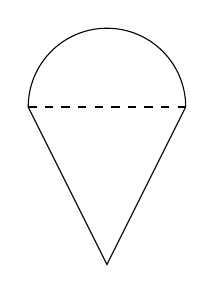
\begin{tikzpicture}
      \draw (-1, 0) arc[radius=1, start angle=180, end angle=0]; %
      \draw[dashed] (-1, 0) -- (1, 0); % 
      \draw (-1, 0) -- (0, -2) -- (1, 0); % 
    \end{tikzpicture}
  \end{problem}  

\end{enumerate}
\end{document}
